\section{Background}

The Boltzmann transport equation can be solved directly in 3D to obtain 3D flux and power distributions.  One method to do this is the 3D Method of characteristics, which is implemented in MPACT \cite{KochunasThesis}.  However, performing these 3D transport calculations becomes too computationally burdensome to be of practical use, even with today's improved computing resources.  Because LWRs have most of their material heterogeneity in the radial direction with very little change in the axial direction, it was recognized that approximations could be made in the axial direction to increase the efficiency of the calculations while still performing high-fidelity transport calculations in the radial direction.  Two different groups of researchers pursued this concept and developed two different methods of solving the transport equation for LWR problems.

The first of these methods was the ``2D/1D Fusion'' technique, developed by researchers at Korea Advanced Institute of Science and Technology (KAIST) and implemented in codes such as CRX \cite{Fusion2D1D,FusionMOC}.  In this method, the 3D problem is decomposed into a stack of 2D planes.  These planes are solved using 2D MOC, with incoming angular fluxes on the top and bottom boundaries of the plane as source terms.  To couple the planes, the problem domain is integrated in the x- and y-directions for each pin cell.  The angular fluxes at the radial edges are obtained from the 2D MOC calculations and used as source terms.  The angular fluxes are then solved in the axial direction using the Diamond Difference \todo{cite} method.  These results, in turn, are fed back into the radial calculations.  Iterating between the radial and axial calculations then produces a full 3D solutions.

The second group of researchers was at Korea Atomic Energy Research Institute (KAERI).  They developed what is known more simply as the ``2D/1D'' scheme, first implemented in the DeCART code \cite{3DHetWholeCoreTransPlanarMOC,DeCARTTheoryManual,MethodsAndPerformanceOfDecart}.  This employs very similar technique to the 2D/1D Fusion method described above.  However, rather than using angular fluxes from each solver as a source term, currents are tallied on each of the six faces of each pin cell.  The currents can then be used to compute axial and radial ``transverse leakage'' sources for the radial and axial solvers, respectively.  This change allows for the storage of group-wise currents at each interface instead of storing the group-wise angular fluxes for each angle, significantly reducing the memory burden of the calculation.

After some development, the DeCART code was forked into several different versions for different institutions, one of them being the University of Michigan (UM).  After some development, it was determined that there would be no further development of the DeCART code at UM and a new 2D/1D implementation would be put in MPACT \cite{2D1DApproxTo3DTransport1,StabilityAndAccuracyOf3DTransportInMPACT}.  In MPACT's implementation of 2D/1D, 2D MOC is used for each of the radial planes, as with earlier 2D/1D codes.  The axial calculation done on a pin-homogenized mesh usually with SP$_3$, though a variety of other solver are available such as NEM \todo{cite}, SENM \todo{cite}, SP$_1$, SP$_5$, or S$_N$.  Finally, MPACT also uses 3D CMFD on the same pin-homogenized mesh to provide convergence acceleration to the calculations.  The remainder of this chapter will look at the derivation of the 2D/1D equations, the details of how they are implemented in MPACT, and some of the approximations and sources of errors related to this method.

\section{Derivation}

\subsection{Radial Equations}

To derive the radial equations, we begin with the multigroup approximation in equation \ref{e:multigroupboltzmann}  and integrate in the $z$-direction over some range $\Delta z_i = z_{k+\frac{1}{2}} - z_{k-\frac{1}{2}}$.  To do this, we assume the cross-sections are all constant in the interval $z \in \left[z_{k-\frac{1}{2}},z_{k+\frac{1}{2}}\right]$.  With this assumption, we obtain the following equation:
\begin{subequations}
\begin{dmath}\label{e:2D1DradialEq}
{\Omega_x\frac{\partial \psi_{g}^Z}{\partial x} + \Omega_y\frac{\partial \psi_{g}^Z}{\partial y} + \frac{\Omega_z}{\Delta z_k}\left(\psi_{g,z_{k+\frac{1}{2}}} - \psi_{g,z_{k-\frac{1}{2}}}\right)} + {\Sigma_{t,g}\left(x,y\right)\psi_{g}^Z\left(x,y,\bm\Omega\right)} = {\frac{1}{4\pi}\sum_{g'=1}^{G}\intop_{4\pi}\Sigma_{s,g'\rightarrow g}^Z\left(x,y,\bm\Omega'\cdot\bm\Omega\right)\psi_{g'}^Z\left(x,y,\bm\Omega'\right)d\Omega'} + {\frac{1}{k_{eff}}\frac{\chi_{g}^Z}{4\pi}\sum_{g'=1}^G\intop_{4\pi} \nu\Sigma_{f,g'}^Z\left(x,y\right)\psi_{g'}^Z\left(x,y,\bm\Omega'\right)d\Omega'} + {\frac{Q_{g}^Z\left(x,y\right)}{4\pi}}
\end{dmath}
\begin{equation}
\psi_g^Z\left(x,y,\bm{\Omega}\right) = \frac{1}{\Delta z_k} \intop_{z_{k-\frac{1}{2}}}^{z_{k+\frac{1}{2}}} \psi_g^Z\left(x,y,z,\bm{\Omega}\right) dz
\end{equation}
\end{subequations}
where a superscript $Z$ indicates the average of a quantity over a given plane.  The $z$-component of the streaming can now be moved to the right-hand side of the equation and treated as a source term, giving a 2D transport problem which could be solved with a variety of methods:
\begin{subequations}
\begin{dmath}
{\Omega_x\frac{\partial \psi_{g}^Z}{\partial x} + \Omega_y\frac{\partial \psi_{g}^Z}{\partial y}} + {\Sigma_{t,g}\left(x,y\right)\psi_{g}^Z\left(x,y,\bm\Omega\right)} = {q_{g}^Z\left(x,y\right) + L_{g}^Z\left(x,y,\Omega_z\right)}
\end{dmath}
\begin{dmath}
q_{g}^Z\left(x,y\right) = {\frac{1}{4\pi}\sum_{g'=1}^{G}\intop_{4\pi}\Sigma_{s,g'\rightarrow g}^Z\left(x,y,\bm\Omega'\cdot\bm\Omega\right)\psi_{g'}^Z\left(x,y,\bm\Omega'\right)d\Omega'} + {\frac{1}{k_{eff}}\frac{\chi_{g}^Z}{4\pi}\sum_{g'=1}^G\intop_{4\pi} \nu\Sigma_{f,g'}^Z\left(x,y\right)\psi_{g'}^Z\left(x,y,\bm\Omega'\right)d\Omega'} + {\frac{Q_{g}^Z\left(x,y\right)}{4\pi}}
\end{dmath}
\begin{equation}
L_{g}^Z\left(x,y,\Omega_z\right) = \frac{\Omega_z}{\Delta z_k}\left(\psi_{g,z_{k-\frac{1}{2}}} - \psi_{g,z_{k+\frac{1}{2}}}\right)
\end{equation}
\end{subequations}
where $L_{g}^Z\left(x,y,\Omega_z\right)$ is the axial transverse leakage source term for plane $z$.  To simplify the source term, the axial transverse leakage term is often handled isotropically.  This is done by averaging over angle:
\begin{equation}
L_{g}^Z\left(x,y\right) = \frac{1}{4\pi}\intop L_{g}^Z\left(x,y,\Omega_z\right) \approx \frac{J_{g,z_{k-\frac{1}{2}}} - J_{g,z_{k+\frac{1}{2}}}}{4\pi\Delta z_k}
\end{equation}
where $J_{z_{i\pm \frac{1}{2}}}$ is the current at the top ($+$) or bottom ($-$) of the plane.  This eliminates the need for storing all the angluar fluxes on the top and bottom of every plane.  Other methods exist that allow the axial transverse leakage source to maintain its angular dependence without storing the angular fluxes\todo{Cite Blake and others}, but these methods are not discussed here since they were not used by this work.

\subsection{Axial Equations}

The axial equations can be derived in a manner similar to the radial equations.  Again, we begin with the multi-group approximation shown in equation \ref{e:multigroupboltzmann}.  This time, we integrate in both the x and y directions over intervals $x \in \left[x_{i-\frac{1}{2}},x_{i+\frac{1}{2}}\right]$ and $y \in \left[y_{j-\frac{1}{2}},y_{j+\frac{1}{2}}\right]$, giving the following equations in the axial direction, which are analogous to the radial equations in the previous section:
\begin{subequations}\label{e:2D1DaxialEq}
\begin{dmath}
{\Omega_z \frac{\partial \psi_{g}^{XY}}{\partial z}} + {\Sigma_{t,g}^{XY}\left(z\right)\psi_{g}^{XY}\left(z,\bm\Omega\right)} = q_{g}^{XY}\left(z,\Omega_x,\Omega_y\right) + {L_{g}^{XY}\left(z,\Omega_x,\Omega_y\right)}
\end{dmath}
\begin{dmath}
q_{g}^{XY}\left(z,\Omega_x,\Omega_y\right) = {\frac{1}{4\pi}\sum_{g'=1}^G\intop_{4\pi} \Sigma_{s,g'\rightarrow g}^{XY}\left(z,\bm\Omega'\cdot\bm\Omega\right)\psi_{g'}^{XY}\left(z,\bm\Omega'\right)d\Omega'} + {\frac{1}{k_{eff}}\frac{\chi_{g}^{XY}}{4\pi}\sum_{g'=1}^G\intop_{4\pi}\nu\Sigma_{f,g'}^{XY}\left(z\right)\psi_{g'}^{XY}\left(z,\bm\Omega'\right)d\Omega'} + {\frac{Q_{g}^{XY}\left(z\right)}{4\pi}}
\end{dmath}
\begin{dmath}
L_{g}^{XY}\left(z,\Omega_x,\Omega_y\right) = {\frac{\Omega_x}{\Delta y_i}\intop_{y_{i-\frac{1}{2}}}^{y_{i+\frac{1}{2}}} \left(\psi_{g,x_{i-\frac{1}{2}}}\left(y\right) - \psi_{g,x_{i+\frac{1}{2}}}\left(y\right) dy\right)} + {\frac{\Omega_y}{\Delta x_i}\intop_{x_{i-\frac{1}{2}}}^{x_{i+\frac{1}{2}}} \left(\psi_{g,y_{i-\frac{1}{2}}}\left(x\right) - \psi_{g,y_{i+\frac{1}{2}}}\left(x\right) dx\right)}
\end{dmath}
\begin{equation}\label{e:2D1DaxFluxDef}
\psi_g^{XY} = \frac{1}{\Delta_i \Delta_j} \intop_{y_{j-\frac{1}{2}}}^{y_{j+\frac{1}{2}}} \intop_{x_{i-\frac{1}{2}}}^{x_{i+\frac{1}{2}}} \psi_g\left(x,y,z,\bm{\Omega}\right) dx dy
\end{equation}
\end{subequations}
where a superscript $XY$ now corresponds to a particular x- and y-region which extends the full height of the problem in the z-direction.  Again, it is assumed that the cross-sections are constant in the x- and y-directions inside the region of integration.  How this is accomplished will be discussed in more detail when discussing MPACT's implementation of SP$_3$ and CMFD.

As with the radial equations, we can treat the transverse leakage source isotropically by averaging over angle:

\begin{dmath}
{L_{g}^{XY}\left(z\right)} = {\frac{1}{4\pi}\intop_{4\pi} L_{g}^{XY}\left(z,\Omega_x,\Omega_y\right)} \approx {\frac{1}{4\pi\\Delta y_i}\intop_{y_{i-\frac{1}{2}}}^{y_{i+\frac{1}{2}}}\left( J_{g,x_{i-\frac{1}{2}},y_i}\left(z\right) - J_{g,x_{i+\frac{1}{2}},y_i}\left(z\right)\right)dy} + {\frac{1}{4\pi\Delta x_i}\intop_{x_{i-\frac{1}{2}}}^{x_{i+\frac{1}{2}}}\left( J_{g,x_i,y_{i-\frac{1}{2}}}\left(z\right) - J_{g,x_i,y_{i+\frac{1}{2}}}\left(z\right)\right)dx}
\end{dmath}

Again, methods have been developed to angle the angle-dependence of the radial transverse leakage source\todo{Cite Shane and anyone else who has done it}, but this work used only isotropic radial leakage.

\section{Implementation}

Now that the general 2D/1D scheme has been described, some attention should be given to the details of its implementation in MPACT.  Figure \ref{f:2d1d-flowchart} shows the calculation flow used by MPACT.  The first step is to perform a global 3D CMFD calculation to obtain pin-averaged flux and interface currents between each cell.  Next, the axial solver uses the radial currents calculated by CMFD as a radial transverse leakage source to obtain an axial transverse leakage source for the radial solver.  Finally, 2D MOC is used as the radial solver to obtain a solution with sub-pin resolution in each plane.

\begin{figure}[h]
  \centering
  \begin{tikzpicture}[node distance=2cm]

% Begin
\node (start) [startstop] {Start};
\node (init) [io, right of=start, xshift=2.0cm] {Input, Initialize Solution};

% CMFD
\node (CMFD) [process, below of=init] {CMFD Eigenvalue Calculation};

% Nodal
\node (Nodal) [process, below of=CMFD] {Axial P$_3$ Calculation};

% MOC
\node (MOC) [process, below of=Nodal] {2D MOC Sweeps};

% Finish
\node (convCheck) [decision, below of=MOC, yshift=-1.5cm] {Fission Source, k-eff Converged?};
\node (out) [io, below of=convCheck,yshift=-1.5cm] {Output};
\node (stop) [startstop, right of=out, xshift=2.0cm] {Stop};

% Basic Arrows
\draw [arrow] (start) -- (init);
\draw [arrow] (init) -- (CMFD);
\draw [arrow] (CMFD) -- (Nodal);
\draw [arrow] (Nodal) -- (MOC);
\draw [arrow] (MOC) -- (convCheck);
\draw [arrow] (out) -- (stop);

% Fancy Arrows
\draw [arrow] (convCheck) -- node[anchor=west] {yes} (out);
\draw [arrow] (convCheck) -| node[anchor=north] {no} ([xshift=1.5cm]Nodal.east) |- (CMFD);

\end{tikzpicture}
  \caption{Calculation flow for 2D/1D scheme}\label{f:2d1d-flowchart}
\end{figure}

Now that the general 2D/1D scheme has been described, some attention should be given to the details of its implementation in MPACT.  Figure \ref{f:2d1d-flowchart} shows the calculation flow used by MPACT.  The first step is to perform a global 3D CMFD calculation to obtain pin-averaged flux and interface currents between each cell.  Next, the axial solver uses the radial currents calculated by CMFD as a radial transverse leakage source to obtain an axial transverse leakage source for the radial solver.  Finally, 2D MOC is used as the radial solver to obtain a solution with sub-pin resolution in each plane.

\subsection{3D Sub-plane CMFD}

\begin{figure}[h]
  \centering
  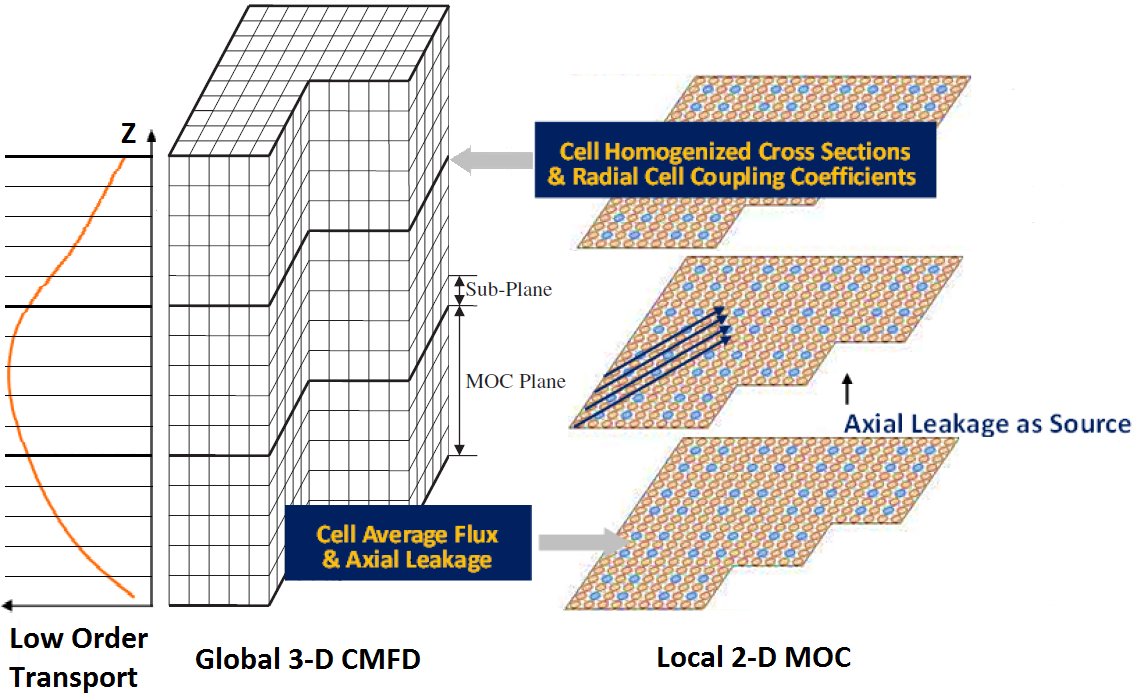
\includegraphics[width=0.8\textwidth]{../figs/2d1d-subplane.png}
  \caption{2D/1D with subplane}
  \label{f:2d1dsubpalne}
\end{figure}

The CMFD method was originally implemented in MPACT just as described in section \ref{ss:CMFD}.  To do this, each pin cell is homogenized using the quantities defined in equation \ref{e:CMFDhomogTerms} in every plane in the model.  The radial coupling coefficients defined in equation \ref{e:CMFDcouplingCoeffs} are obtained by calculating the current at the interface between each pair of pin cells using the 2D MOC sweeper, while the axial coupling coefficients are obtained from the axial currents calculated by the axial solve during the previous iteration.  The matrix for the 3D multi-group system can then be set up and solved, typically using the generalized Davidson eigenvalue solver.

In addition to this traditional 3D CMFD, MPACT also has the capability to use the sublpane scheme \cite{DeCARTsubplane,ICAPPcontrolRodDecuspingNTRACER}.  This scheme was first implemented in the DeCART code to allow users to increase the thickness of the 2D planes while still maintaining the accuracy of a fine axial mesh.  This eliminated some convergence difficulties associated with thin 2D planes \todo{citation?} and reduced the computational burden of performing MOC on many thin planes.  However, the sub-plane scheme is also being employed as a framework to develop new control rod decusping methods (discussed in more detail in chapter \ref{chap:cusping}).


\subsubsection{Homogenization}

The difference between the sub-plane scheme and traditional CMFD is that the CMFD system is that the CMFD system is allowed to have multiple axial planes for each of the 2D planes in which the transport calculations are done.  This allows CMFD to capture sub-plane axial flux shapes that would otherwise be ignored.  To do this, a sub-plane scaling factor is introduced which will be used to provide an axial shape within a 2D plane:

\begin{align}
c_{g,i}^k &= \frac{\phi_{g,i}^{k-1}}{\overline{\phi}_{g,i}^{k-1}} \nonumber\\
 &= \frac{\phi_{g,i}^{k-1} \sum_{i'=1}^{N_{sp}} V_{i'}}{\sum_{i'=1}^{N_{sp}} \phi_{g,i'}^{k-1} V_{i'}}
\end{align}

where superscripts indicate which iteration the values are taken from and $N_{sp}$ is the number of sub-planes for the pin cell of interest.  Now when the homogenized values are calculated from the 2D transport solution using equation \ref{e:CMFDhomogTerms}, the fine mesh flux is multiplied by this sub-plane scaling factor everywhere it appears.  Because the 2D/1D scheme assumes a constant material axially in each plane, this sub-plane factor has no impact on the homogenized cross-sections.  However, the homogenized flux $\phi_{g,i}$ and fission source distribution $\chi_{g,i}$ will be changed, providing an axial shape for the source term in the eigenvalue calculation.

\subsubsection{Coupling Coefficients}

In addition to the homogenized cell terms, the coupling coefficients described by equations \ref{e:CMFDinterface} and \ref{e:CMFDcouplingCoeffs} must be calculated for each sublpane.  To maintain consistency, the area-averaged current calculated by the radial sweeper must be preserved across the sub-surfaces used by the sub-plane scheme.  Thus, the current calculated by the radial sweeper at an interface is used at the corresponding interfaces for all sub-planes in that plane.  Additionally, to maintain consistency, this requires that the cell-homogenized flux used in the calculation of the diffusion coefficients be defined for the entire MOC plane as in equation \ref{e:CMFDhomogFlux} rather than using the sub-plane scaling factor for each sub-plane.

The axial coupling coefficient can be treated in a more straightforward manner.  Because the 1D axial solvers use the same pin-homogenized mesh as the CMFD solver, axial currents are naturally calculated at the top and bottom of each of the sub-planes.  Thus, these currents can be used together with the sub-planes fluxes to calculate sub-plane--dependent axial coupling coefficients.

\subsubsection{Projection}

The projection of the CMFD flux back to the 2D planes must also account for the presence of the sub-planes.  To do this, the solution is volume-averaged over all sub-planes for each pin cell, resulting in an equation similar to \ref{e:CMFDscaling}:

\begin{equation}
\phi_{trans,g,j}^k = \frac{\sum_{i'=1}^{N_{sp}} \phi_{CMFD,g,i'}^k V_i}{\sum_{i'=1}^{N_{sp}} \phi_{CMFD,g,i'}^k V_i} \phi_{trans,g,j}^{k-1}
\end{equation}

The calculation flow for 3D CMFD is shown in figure \ref{f:CMFD-flowchart}.

\begin{figure}[h]
  \centering
  \begin{tikzpicture}[node distance=2cm]

% Start
\node (start) [startstop] {Start};

% CMFD
\node (homog) [process, right of=start, xshift=2.0cm] {Homogenize Cross-sections and Flux; Calculate $\tilde{D}$};
\node (iterCheck) [decision, below of=homog, yshift=-1.5cm] {First Iteration?};
\node (firstIter) [process, below of=iterCheck, xshift=-2.5cm, yshift=-1.0cm] {Set $\hat{D}=0$};
\node (laterIter) [process, below of=iterCheck, xshift=2.5cm, yshift=-1.0cm] {Calculate $\hat{D}$};
\node (matrix) [process, below of=firstIter, xshift=2.5cm] {Set up CMFD Matrix};
\node (3DCMFD) [process, below of=matrix] {3D CMFD Calculation};
\node (proj) [process, below of=3DCMFD] {Scale MOC flux with CMFD flux};

% Stop
\node (stop) [startstop, right of=proj, xshift=2.0cm] {Stop};

% Basic Arrows
\draw [arrow] (start) -- (homog);
\draw [arrow] (homog) -- (iterCheck);
\draw [arrow] (matrix) -- (3DCMFD);
\draw [arrow] (3DCMFD) -- (proj);
\draw [arrow] (proj) -- (stop);

% Fancy Arrows
\draw [arrow] (iterCheck) -| node[anchor=south] {yes} (firstIter);
\draw [arrow] (iterCheck) -| node[anchor=south] {no} (laterIter);
\draw [arrow] (firstIter) |- (matrix);
\draw [arrow] (laterIter) |- (matrix);

\end{tikzpicture}
  \caption{Calculation flow for 3D sub-plane CMFD}\label{f:CMFD-flowchart}
\end{figure}

\subsection{1D Axial}

In MPACT, the 1D axial solvers operate on the same mesh as the 3D CMFD calculations, meaning that cell-homogenized quantities and radial currents have already been obtained from the CMFD calculation.  All the 1D axial solver must do is construct a source term from the radial currents for each cell, then perform a calculation to obtain currents on the axial interfaces at the top and bottom of each node.

MPACT has a variety of 1D nodal methods that are capable of performing these calculations, including diffusion-based such as NEM and SENM and higher-order solvers such as SP$_N$ and S$_N$.  For most MPACT calculations, including those in this work, the solver of choice is SP$_3$, which provides significant improvement over the diffusion-based methods and SP$_1$.  Very little benefit is obtained by using the higher-order SP$_5$\todo{citation}.

\begin{figure}[h]
  \centering
  \begin{tikzpicture}[node distance=2cm]

% Begin
\node (start) [startstop] {Start};

% Nodal
\node (radialTL) [process, right of=start, xshift=2.5cm] {Calculate radial transverse leakage source};
\node (sp3-0) [process, below of=radialTL] {Solve 0th moment equation};
\node (sp3-2) [process, below of=sp3-0] {Solve 2nd moment equation};
\node (convCheck) [decision, below of=sp3-2, yshift=-1.5cm] {Converged?};

% Stop
\node (stop) [startstop, right of=convCheck, xshift=2.5cm] {Stop};

% Basic Arrows
\draw [arrow] (start) -- (radialTL);
\draw [arrow] (radialTL) -- (sp3-0);
\draw [arrow] (sp3-0) -- (sp3-2);
\draw [arrow] (sp3-2) -- (convCheck);
\draw [arrow] (convCheck) -- node[anchor=north] {yes} (stop);

% Fancy Arrows
\draw [arrow] (convCheck) -| node[anchor=north] {no} ([xshift=-1.5cm]sp3-2.west) |- (sp3-0);

\end{tikzpicture}
  \caption{Calculation flow for 1D axial calculations in MPACT}\label{f:Axial-flowchart}
\end{figure}

\subsection{2D MOC}

For the radial calculations, 2D MOC is used.  This allows MPACT to easily calculate scalar fluxes and currents in each plane regardless of the geometric complexity.  This section is devoted to discussing some of the details of the MOC implementation and sweeping algorithm in MPACT.

\subsubsection{Ray Tracing}

One of the key features of MPACT's MOC implementation is that of modular ray tracing.  Ray tracing is performed once at the beginning of a calculation and stored for the remainder of the calculation.  Doing this greatly reduces the runtime of the MOC sweeps since the length of each ray segment and the region it is crossing are already known ahead of time.  Furthermore, MPACT takes advantage of the repeatable nature of a reactor's geometry.  Because reactor geometry is repetitive, small portions of the geometry which repeat frequently can be ray-traced separately instead of tracing the entire core.  These smaller units of geometry are known as ray tracing modules, and in MPACT can be a full fuel assembly, a quarter fuel assembly, or a single fuel pin.  After the unique modules are identified, each of them is ray-traced in such a way that the endpoints of a ray in each module will line up with the beginning of a ray in the neighboring module.  This significantly reduces the storage requirements for the ray data since a small number of ray tracing modules can represent a full core problem.

\todo{angle/spacing corrections and volume corrections}

\begin{figure}
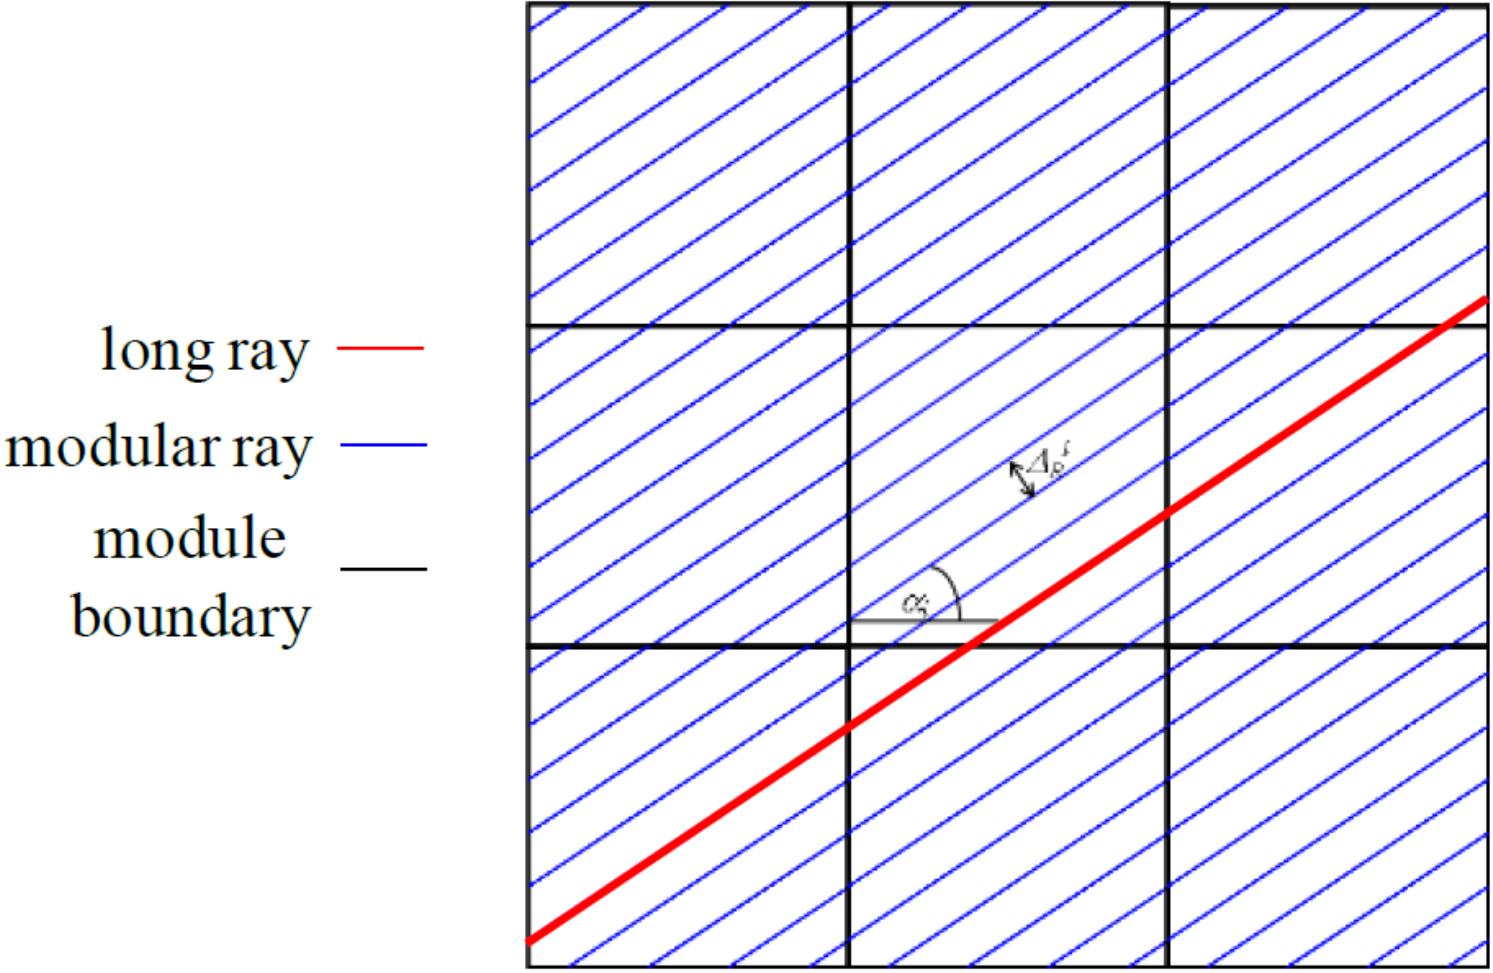
\includegraphics[width=0.5\textwidth]{modular_rays.png}
\caption{Modular Ray Tracing}\label{e:ModRays}
\end{figure}

\subsubsection{Sweeping Algorithm}

\begin{figure}
  \centering
  \begin{tikzpicture}[node distance=2cm]

% Begin
\node (start) [startstop] {Start};
\node (init) [io, right of=start, xshift=2.5cm] {Input N$_{inners}$};

% MOC
\node (begin) [process, below of=init] {Set $n=0$};
\node (source) [process, below of=begin] {Calculate fission and axial transverse leakage sources};
\node (scatSource) [process, below of=source] {Calculate scattering source};
\node (MOC) [process, below of=scatSource] {2D MOC sweep over each energy group};
\node (MOCdone) [decision, below of=MOC, yshift=-1.5cm] {$n = N_{inners}$?};z
\node (stop) [startstop, right of=MOCdone, xshift=2.5cm] {Stop};

% Basic Arrows
\draw [arrow] (start) -- (init);
\draw [arrow] (init) -- (begin);
\draw [arrow] (begin) -- (source);
\draw [arrow] (source) -- (scatSource);
\draw [arrow] (scatSource) -- (MOC);
\draw [arrow] (MOC) -- (MOCdone);

% Fancy Arrows
\draw [arrow] (MOCdone) -| node[anchor=north] {no} ([xshift=-1.5cm]MOC.west) |- (scatSource);
\draw [arrow] (MOCdone) -- node[anchor=north] {yes} (stop);

\end{tikzpicture}
  \caption{Calculation flow for 2D MOC calculation in MPACT}\label{f:MOC-flowchart}
\end{figure}

\section{Parallel Decomposition}

While the 2D/1D scheme greatly reduces runtime from a direct 3D transport calculation, it is still computationally expensive when compared to nodal methods traditionally used by industry.  To minimize the walltime required for 2D/1D calculations in MPACT, several different methods of decomposing the problem for parallel execution have been implemented.  These methods allow MPACT to easily scale to hundreds or thousands of CPUs.  Each of these methods will be briefly described in this section.

\begin{enumerate}[leftmargin=*]
\item \textbf{Spatial Decomposition}

When using this decomposition, each parallel process only has a portion of the model.  Each portion is solved locally by one process, then boundary data is communicated to all processes which own neighboring portions of the model.  The updated boundary data is then used in the following iteration.  When using spatial decomposition, planar decomposition is performed first.  This means that if the total number of parallel processes being used is less than or equal to the number of 2D MOC planes, then one or more entire planes is simulated by each process.  If more processes are used than there are planes in the model, then radial decomposition is performed.  This decomposes every plane radially into smaller pieces.  Every plane must be radially decomposed in the same way, and the smallest unit allowed in radial decomposition is a single ray-tracing module.  Because spatial decomposition does not duplicate much memory and does not decrease the computational efficiency significantly, it is usually the preferred choice of decomposition methods.

\item \textbf{Angle Decomposition}

For angle decomposition, each process has the entire spatial domain.  When the MOC sweeps are performed, each process only sweeps a subset of the angles in the selected quadrature.  After the sweep, a reduction is performed to get the actual scalar flux and currents on all processes.  For the CMFD calculation, the angle processes are re-purposed as spatial processes.  Each angle process owns the full domain, but only solves a portion of it as if it were spatially decomposed.

It is possible to use both spatial and angle decomposition together.  When this is done, spatial decomposition is performed first, then angle decomposition is done within each spatial domain.  In general, the efficiency of angle decomposition calculations is less than that of spatial decompositions.  Furthermore, it also requires that each angle process models all of the spatial domain, increasing the total memory required for the calculation compared with finer spatial decomposition.  However, angle decomposition is still useful for reducing the runtime of cases where further spatial decomposition is not possible.

\item \textbf{Ray Decomposition}

A third type of decomposition that can be done is to decompose the rays in the MOC calculation.  Unlike the previous methods, the ray decomposition makes use of OpenMP threading\todo{cite} instead of MPI.  While performing the MOC sweeps, several threads are used to solve all the rays in each angle.  For the CMFD calculation, MPACT has internal RBSOR solvers which are capable of using threading\todo{cite}.  However, when third-party libraries are used for the CMFD calculations, the threading will be used only during the CMFD calculation.  Threading can also be combined with both spatial and angle decomposition to further increase the parallelism of MPACT.

\item \textbf{Energy Decomposition}

At this time, energy decomposition is not available in MPACT.  However, when it is added, it will be similar to the angle decomposition.  For the MOC calculation, each process will solve a subset of the energy groups on the spatial domain, and for the CMFD calculation, the energy processes will be repurposed as space processes.
\end{enumerate}

\section{Sources of Error}

\begin{enumerate}[leftmargin=*]
\item \hl{Ray Spacing}
\item \hl{Radial Meshing}
\item \hl{Axial Meshing}
\item \hl{Axial TL Spatially flat}
\item \hl{Axial TL Isotropic}
\item \hl{Radial TL Spatially flat}
\item \hl{Radial TL Isotropic}
\item \hl{Scattering}
\item \hl{XS Library}
\item \hl{Axial Homogenization}
\item \hl{Quadrature}
\item \hl{Self-Shielding}
\end{enumerate}

\subsection{Axial Homogenization}

One assumption made in the 2D/1D scheme is that each of the 2D planes is axially homogeneous.  In many cases this assumption is true.  Other times, materials such as spacer grids, end plugs for fuel rods and control tips, or other structural materials may be homogenized, but do not have a large impact on the results, making the axial homogenization within a plane a reasonable approximation.  However, when strongly absorbing materials (or others which may significantly impact neutron behavior) are partially inserted into an axial plane, homogenizing them axially can produce large errors in the solution.  When this occurs, the best way to remedy these errors is to divide the plane into 2 or more planes in such a way that the problematic material is no longer partially inserted into a plane.

While there is a known workaround for this approximation, it has the drawback of adding extra planes to the 2D/1D scheme, which in turn increases the computational burden of the calculations.  Because of this, other methods to improve the axial homogenization have been a topic of interest for reactor components that commonly cause this problem, such as control rods.  This will be discussed in more detail in chapter \ref{chap:cusping}.

\subsection{Axial Transverse Leakage Source}

Another significant approximation in 2D/1D relates to the axial transverse leakage source used by the 2D transport solver.  The 1D axial solve and 3D CMFD acceleration are both done on a pin-homogenized coarse mesh.  This results in the assumption that the axial currents are the same in each part of the pin.  Obviously, this is not true since the fuel and moderator regions will have different energy spectra, thus different currents.  This assumption introduces error in source used in the 2D transport calculations.

\subsection{Radial Transverse Leakage Source}
